\section{\textbf{Simulation}}\label{sec:3}

\begin{figure}[t]
% \centering
% \begin{subfigure}[b]{0.4\textwidth}
    % \centering%
    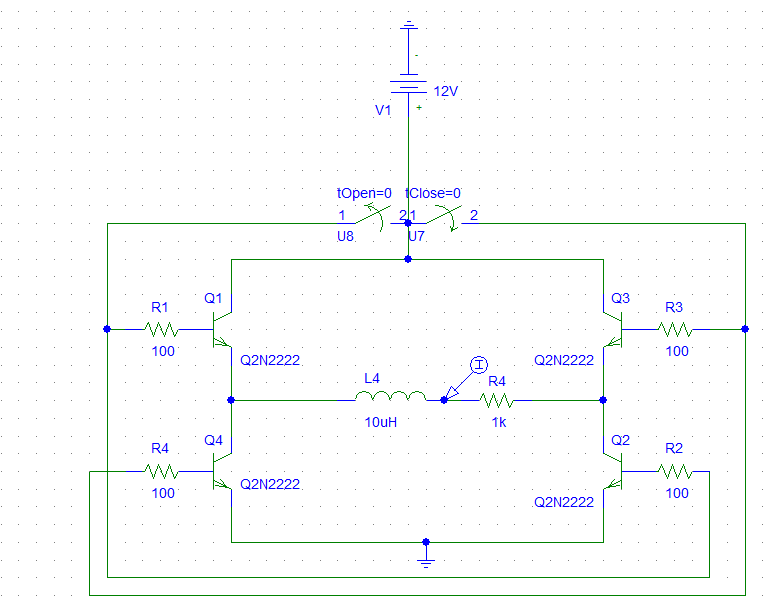
\includegraphics[height=.5\textwidth]{img/schem_pspice.png}
    \caption{Schematic on PSpice program.}\label{fig:schem_pspice}%
% \end{subfigure}\hfill
\end{figure}

    The circuit design was simulated using PSpice software distributed by OrCAD. The circuit shown in Figure~\ref{fig:schem} was reproduced in PSpice (see Figure \ref{fig:schem_pspice}). The software does not support the transistor model used in the actual implementation \todo{add transistor model} instead the Q2N2222 was used to replace it given they are very similar, only the maximum supported values for voltages change. The value of all transistors base resistances was set to $100\:\Omega$. The DC motor simplified equivalent circuit is an inductor and a resistor \todo{ref chapman}. The U8 and U7 times were set to 500 ms.

	Finally a transient analysis over the circuit was made and the current flowing through the motor is plotted in Figure~\ref{fig:plot_ponteh}.
	
	\todo{finish him}
	
\begin{figure}
\centering
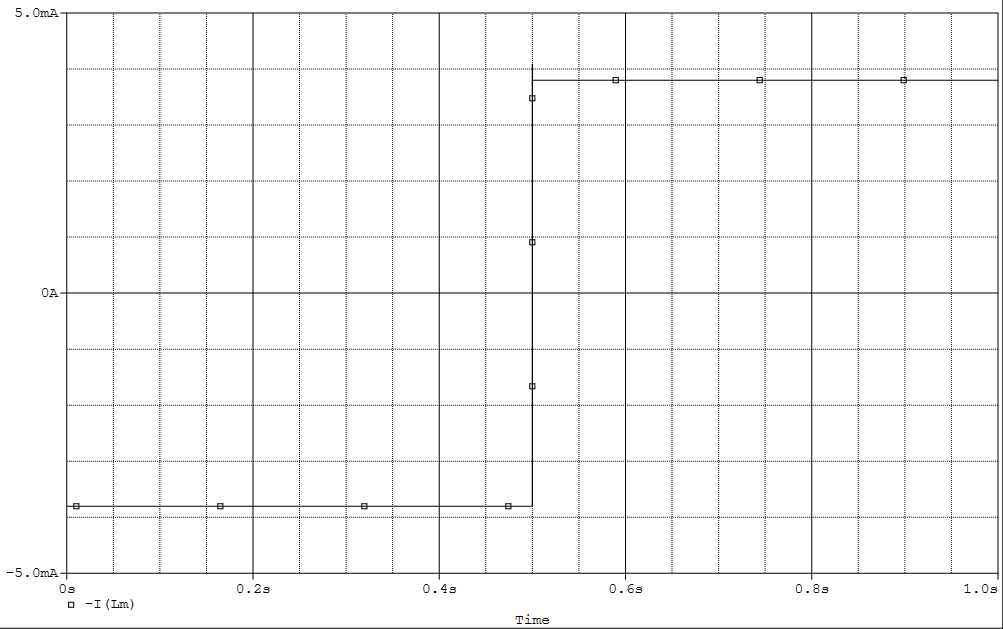
\includegraphics[height=.5\textwidth]{img/plot.png}
\caption{Current x Time} \label{fig:plot_ponteh}
\end{figure}	
